\section{Diagrammi riassuntivi dei package}
Di seguito sono riportati tutti i package dell’applicativo per chiarire la relazione tra le componenti e le classi al suo interno. Per chiarezza ed esigenza di spazio le classi rappresentate all’interno dei package sono rappresentate senza metodi e attributi.


\subsection{Back-end}
Package contenente tutte le componenti che costituiscono il back-end. Le componenti sono organizzate secondo il pattern a microservizi.
\begin{figure}[h] \centering 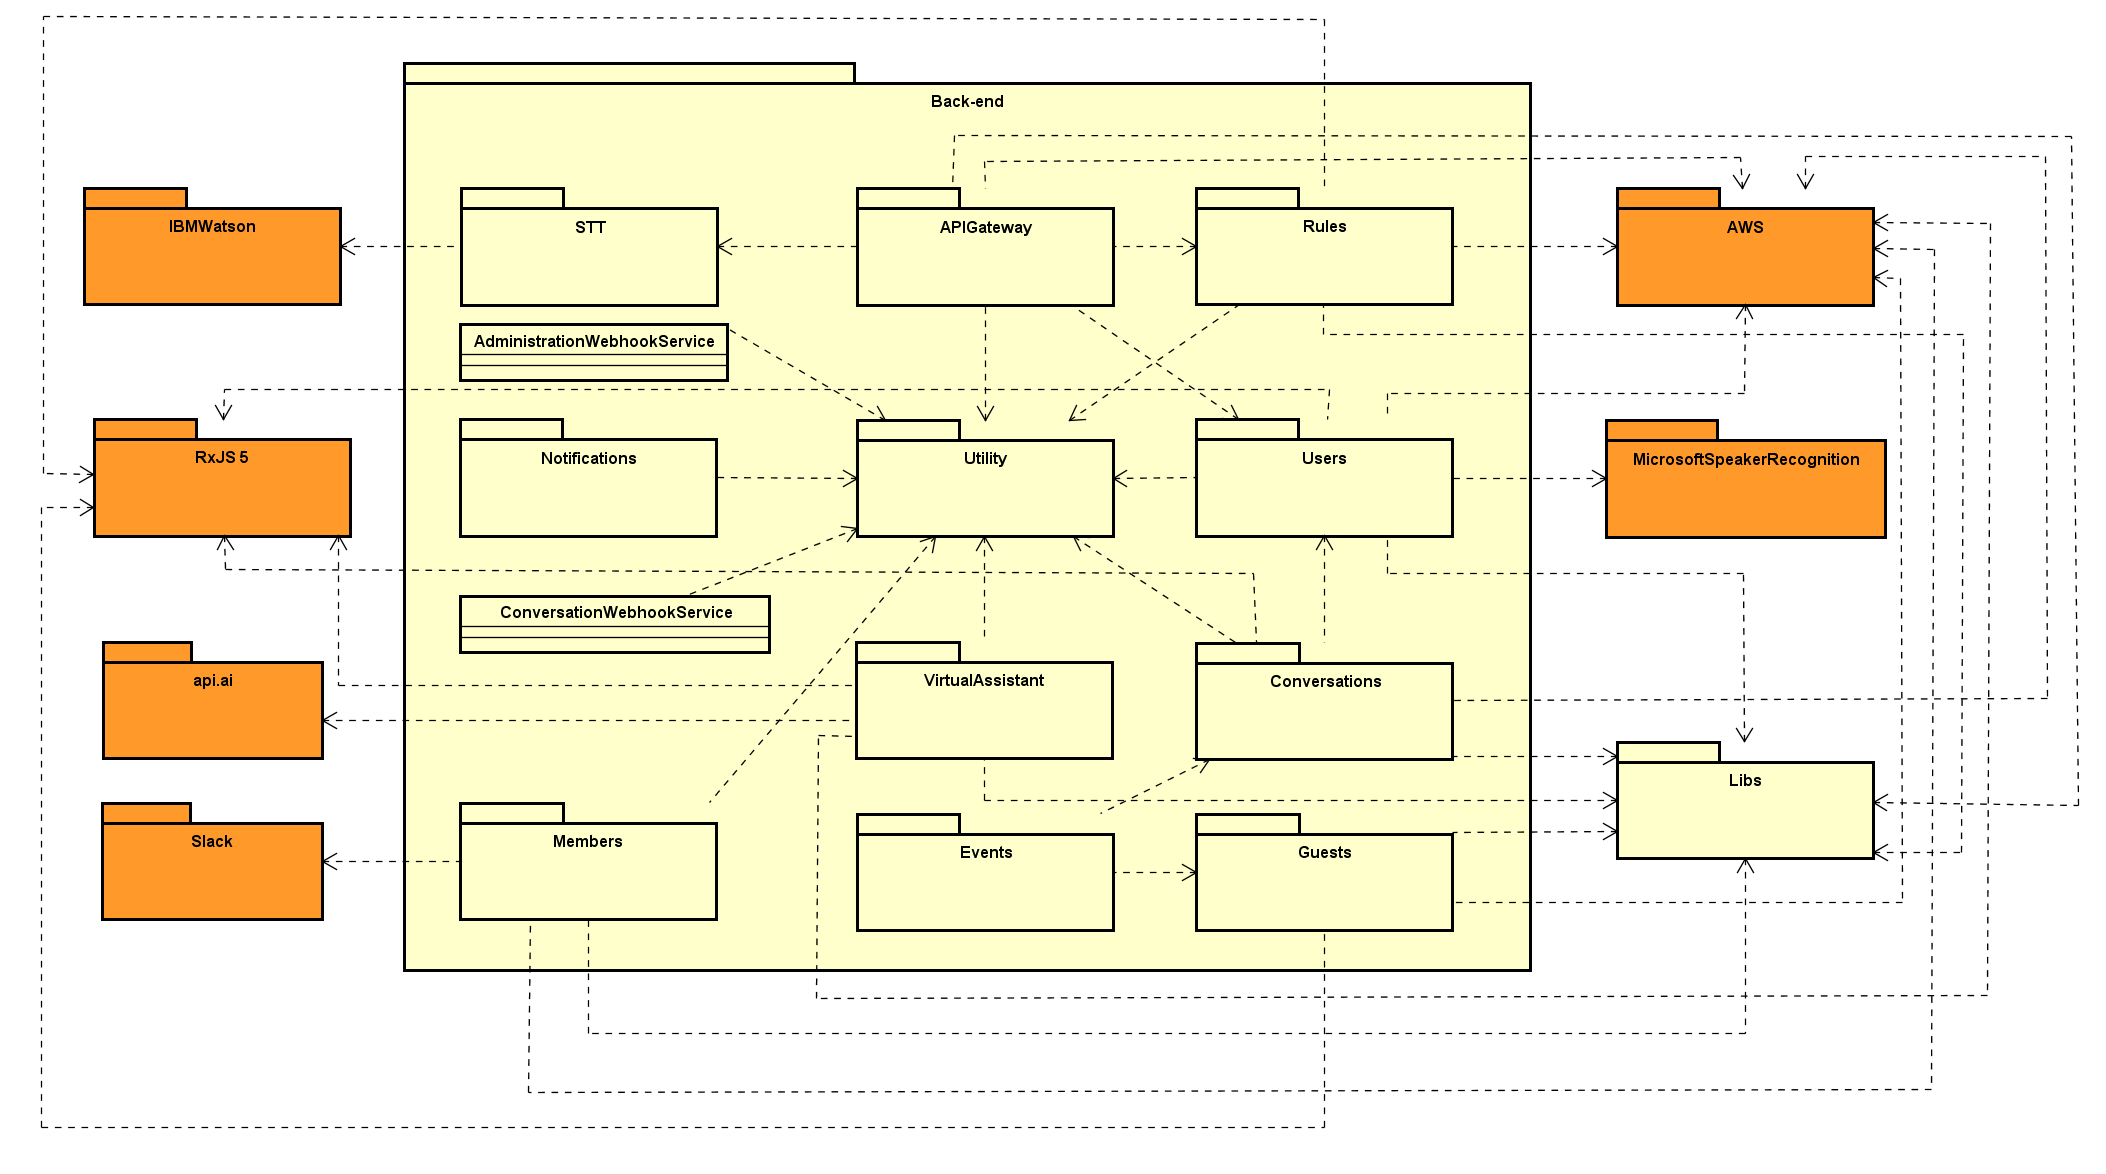
\includegraphics[width=\textwidth,height=\textheight,keepaspectratio]{images/diagrams/back-end/Official_Backend_0304/Back-end.png}
\caption{Package Back-end}
\end{figure}
\newpage

\subsection{Back-end::APIGateway}
Package contenente le classi necessarie a gestire: \begin{itemize} \item diversi tipi di dispositivi client; \item l'interazione tra \file{Client} e \file{Back-end}; \item la combinazione tra i servizi supportati dal \file{Back-end}. \end{itemize}
\begin{figure}[h] \centering 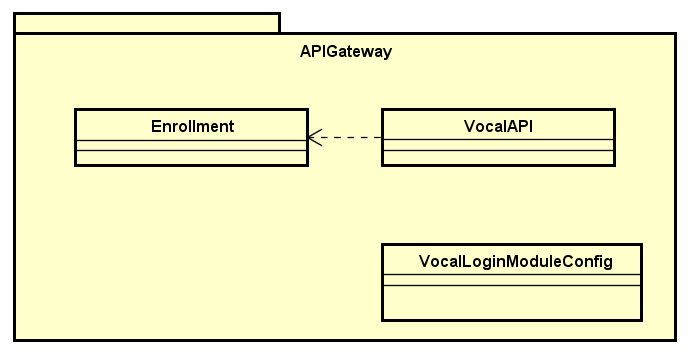
\includegraphics[width=\textwidth,height=\textheight,keepaspectratio]{images/diagrams/back-end/Official_Backend_0304/APIGateway.png}
\caption{Package Back-end::APIGateway}
\end{figure}
\newpage



\subsection{Back-end::Conversations}
Package contenente le classi relative alle Conversations del sistema.
\begin{figure}[h] \centering 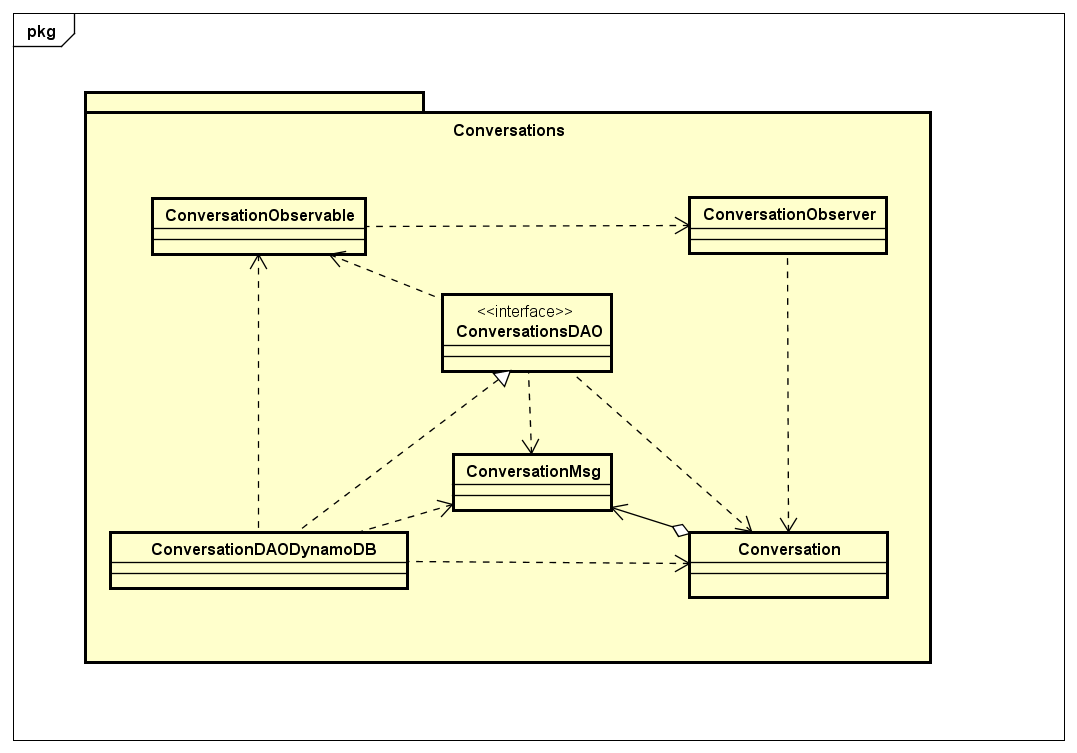
\includegraphics[width=\textwidth,height=\textheight,keepaspectratio]{images/diagrams/back-end/Official_Backend_0304/Conversations.png}
\caption{Package Back-end::Conversations}
\end{figure}
\newpage

\subsection{Back-end::Events}
Package contenente le classi relative alla pubblicazione di eventi all'interno del sistema.
\begin{figure}[h] \centering 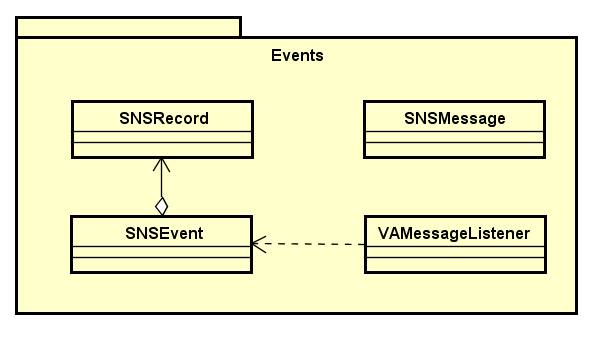
\includegraphics[width=\textwidth,height=\textheight,keepaspectratio]{images/diagrams/back-end/Official_Backend_0304/Events.png}
\caption{Package Back-end::Events}
\end{figure}
\newpage

\subsection{Back-end::Guests}
Package contenente le classi relative ai Guests del sistema
\begin{figure}[h] \centering 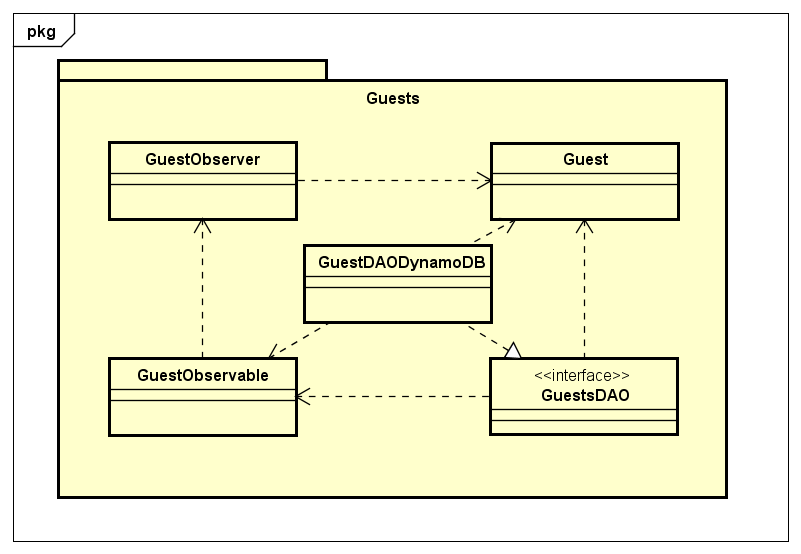
\includegraphics[width=\textwidth,height=\textheight,keepaspectratio]{images/diagrams/back-end/Official_Backend_0304/Guests.png}
\caption{Package Back-end::Guests}
\end{figure}
\newpage

\subsection{Back-end::Members}
Package contenente le classi relative ai membri del sistema
\begin{figure}[h] \centering 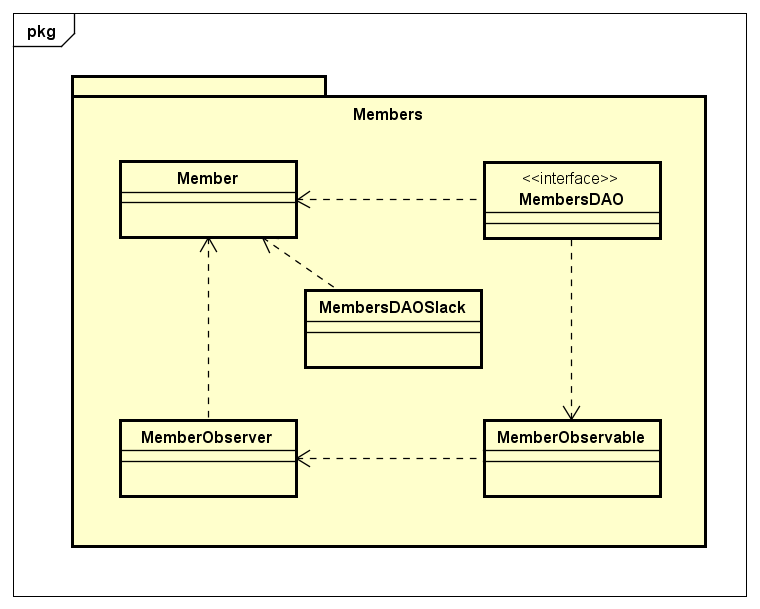
\includegraphics[width=\textwidth,height=\textheight,keepaspectratio]{images/diagrams/back-end/Official_Backend_0304/Members.png}
\caption{Package Back-end::Members}
\end{figure}
\newpage

\subsection{Back-end::Notifications}
Package contenente le classi e le interfacce che realizzano il microservizio relativo alla gestione delle notifiche da inviare alla persona desiderata su una certa piattaforma di messaggistica.
\begin{figure}[h] \centering 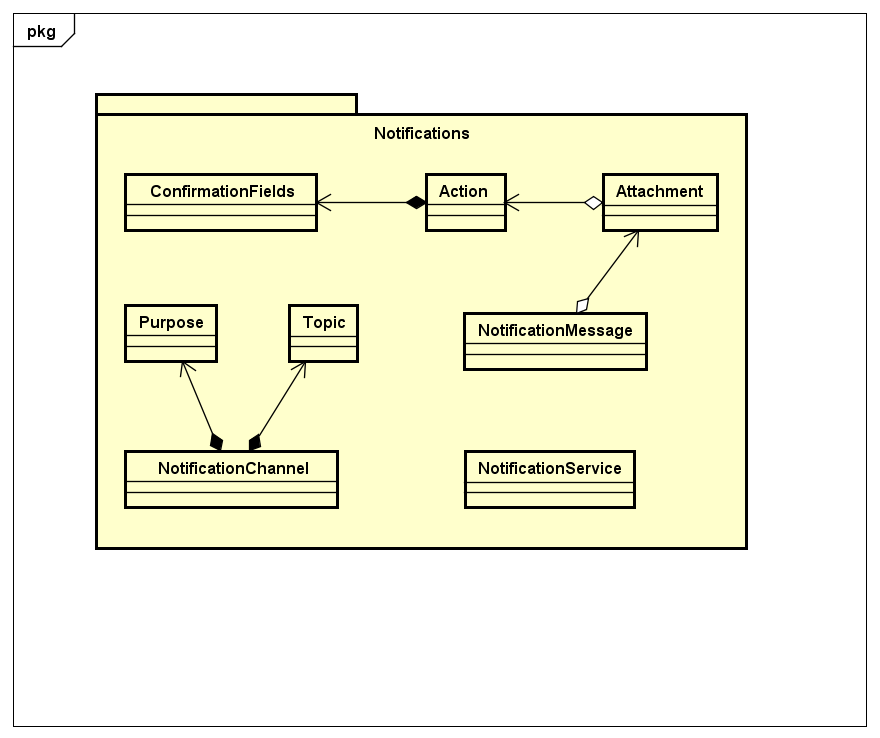
\includegraphics[width=\textwidth,height=\textheight,keepaspectratio]{images/diagrams/back-end/Official_Backend_0304/Notifications.png}
\caption{Package Back-end::Notifications}
\end{figure}
\newpage

\subsection{Back-end::Rules}
Package contenente le classi e le interfacce che realizzano il microservizio di gestione delle direttive per l'assistente virtuale.\\ Vengono offerte funzionalità che permettono: \begin{itemize} \item l'aggiunta di una nuova direttiva; \item l'aggiunta di un nuovo compito (\file{Task}) che una direttiva deve eseguire; \item la gestione delle direttive esistenti; \item la gestione dei compiti esistenti. \end{itemize}
\begin{figure}[h] \centering 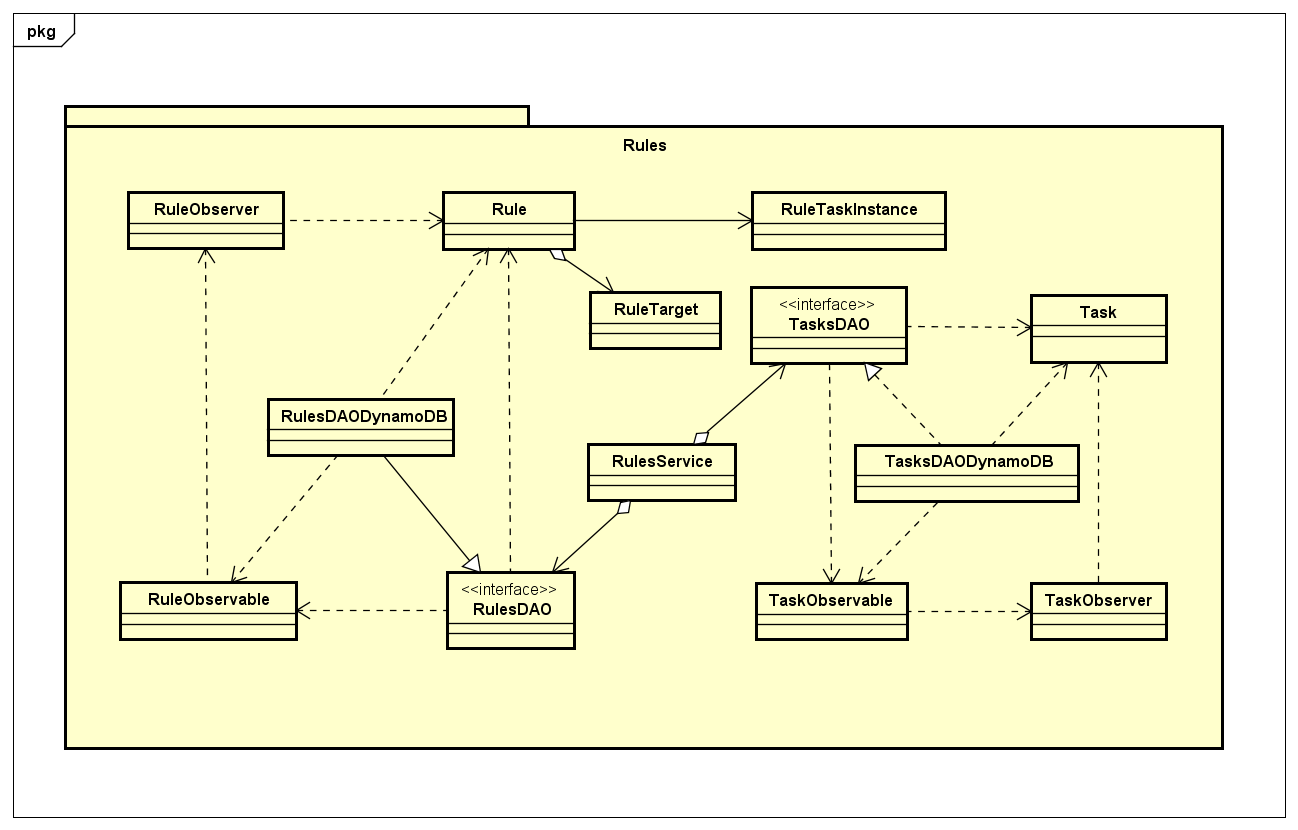
\includegraphics[width=\textwidth,height=\textheight,keepaspectratio]{images/diagrams/back-end/Official_Backend_0304/Rules.png}
\caption{Package Back-end::Rules}
\end{figure}
\newpage

\subsection{Back-end::STT}
Package che include le classi che si occupano di fornire le funzionalità di Speech to text.
\begin{figure}[h] \centering 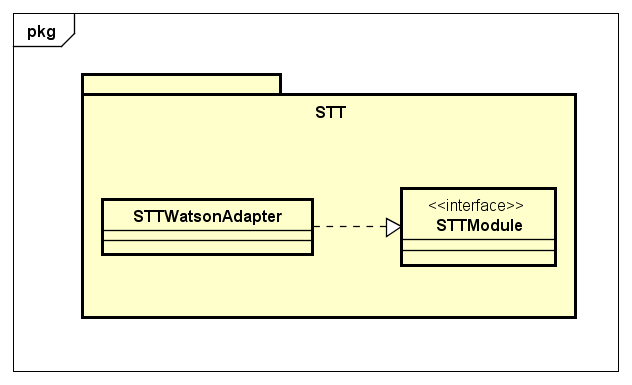
\includegraphics[width=\textwidth,height=\textheight,keepaspectratio]{images/diagrams/back-end/Official_Backend_0304/STT.png}
\caption{Package Back-end::STT}
\end{figure}
\newpage

\subsection{Back-end::Users}
Package contenente le classi e le interfacce che realizzano il microservizio di autenticazione e registrazione di un amministratore nel sistema.\\ Vengono offerte funzionalità che permettono: \begin{itemize} \item la registrazione di un nuovo amministratore; \item l'autenticazione di un amministratore; \item gestione degli amministratori esistenti. \end{itemize}
\begin{figure}[h] \centering 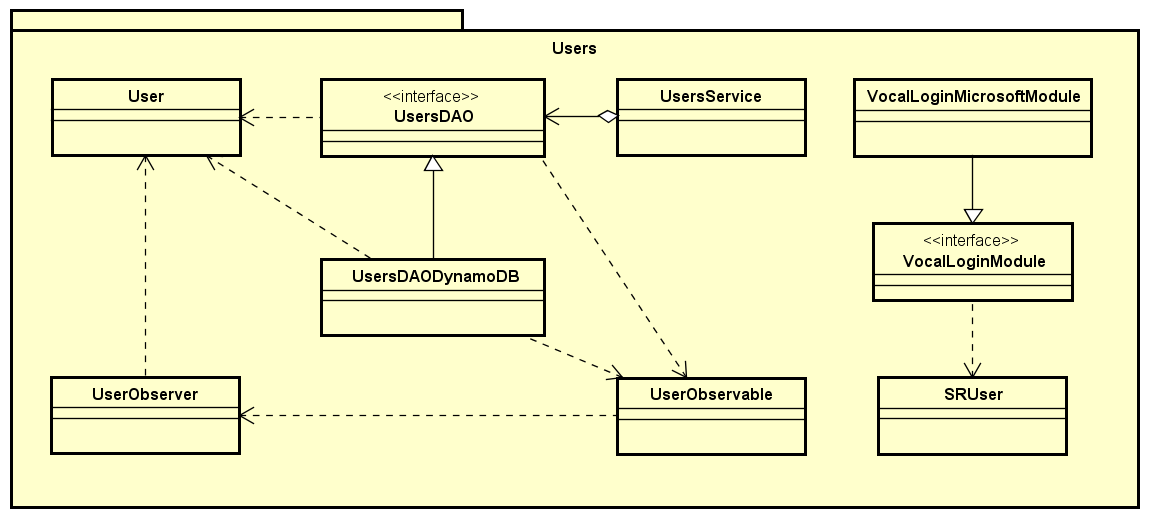
\includegraphics[width=\textwidth,height=\textheight,keepaspectratio]{images/diagrams/back-end/Official_Backend_0304/Users.png}
\caption{Package Back-end::Users}
\end{figure}
\newpage

\subsection{Back-end::Utility}
Package contenente classi e interfacce, dallo scopo generico, utili ad altri package del back-end
\begin{figure}[h] \centering 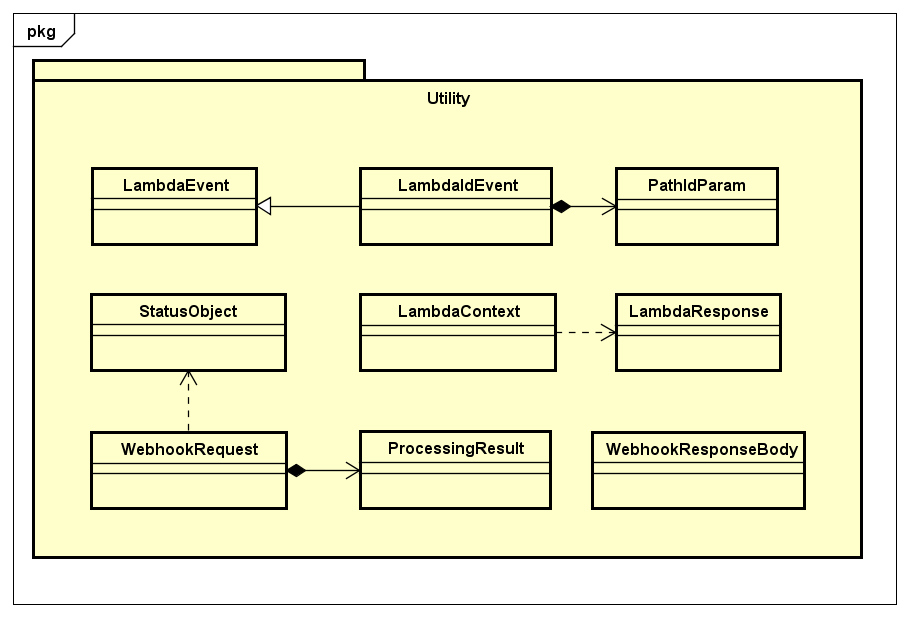
\includegraphics[width=\textwidth,height=\textheight,keepaspectratio]{images/diagrams/back-end/Official_Backend_0304/Utility.png}
\caption{Package Back-end::Utility}
\end{figure}
\newpage

\subsection{Back-end::VirtualAssistant}
Package contenente le classi e le interfacce che realizzano il microservizio di assistente virtuale .\\ Vengono offerte funzionalità che permettono di: \begin{itemize} \item interrogare l'assistemte virtuale. \end{itemize}
\begin{figure}[h] \centering 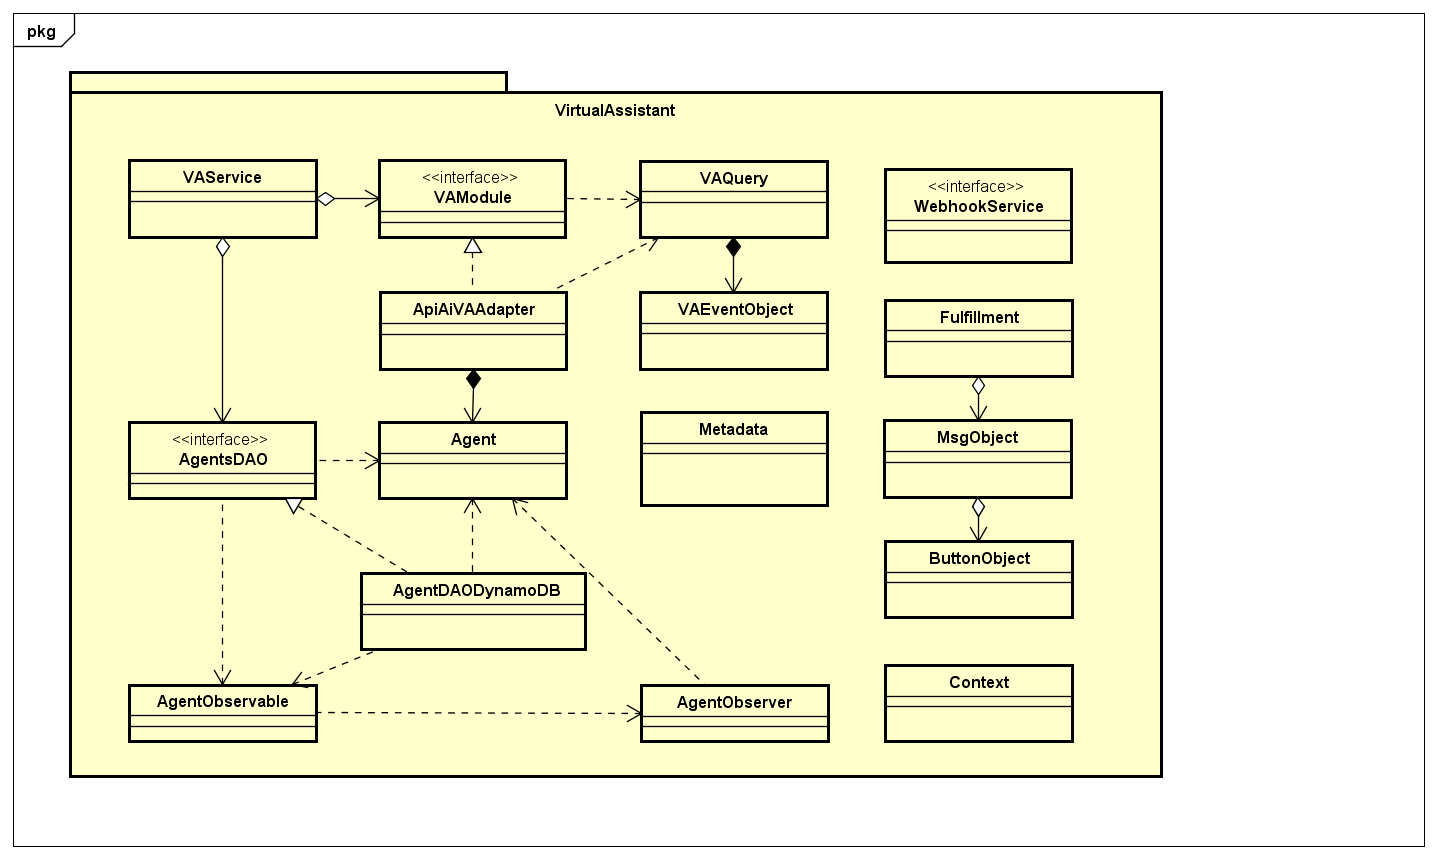
\includegraphics[width=\textwidth,height=\textheight,keepaspectratio]{images/diagrams/back-end/Official_Backend_0304/VirtualAssistant.png}
\caption{Package Back-end::VirtualAssistant}
\end{figure}
\newpage
